\chapter{Tecnologias e Ferramentas Utilizadas}
% OU \chapter{Trabalhos Relacionados}
% OU \chapter{Engenharia de Software}
% OU \chapter{Tecnologias e Ferramentas Utilizadas}
\label{chap:tecnologias_ferramentas_utilizadas}

\section{Introdução}
\label{chap3:sec:intro}
Neste capítulo, são abordadas as ferramentas que foram utilizadas para a construção dos \textit{assets}, assim como também é feito um \textit{overview} do motor de jogo, de maneira a transmitir uma ideia da filosofia e funcionamento geral destas ferramentas.


\section{Blender}
\label{chap3:sec:blender}
Nesta secção, explica-se no que consiste e o processo de criação englobado pela aplicação, apresentando uma opinião pessoal da experiência e aprendizagem com a ferramenta. Expõem-se o trabalho realizado ao utilizar a mesma.

\subsection{Funcionalidades e capacidades}
\label{chap3:subsec:funcionalidades}
Por definição, o \emph{Blender} [4] é uma ferramenta de criação de modelos de computador 3D usada para criar filmes animados, efeitos visuais, modelos para impressão 3D e \textit{assets} para jogos de vídeo.
Inclui funcionalidades para modelação, renderização, rasterização, \textit{rigging} e simulações de corpos físicos complexos, como fumo e fluídos. Compreende um motor de jogo próprio.

\subsection{Experiência}
\label{chap3:subsec:experiencia}
Anteriormente à realização do projeto, o contato com a ferramenta era inexistente. Foi, portanto, necessário um processo de aprendizagem para produzir modelos satisfatórios para uso na aplicação. Esta evolução pode ser notada na crescente qualidade dos modelos, sendo este o pretendido. Desta forma, consegue-se formar uma explicação do processo de evolução que pode ser facilmente entendida e verificada.\\


O primeiro passo passou pela familiarização com a interface da ferramenta e com as funcionalidades que esta apresenta. Após este primeiro passo, foi iniciado o desenvolvimento de formas 3D simples, de modo a perceber várias metodologias para adicionar detalhe e dimensão a estas. Obtendo-se o conhecimento elementar para a produção de modelos com qualidade satisfatória, procedeu-se à produção do primeiro modelo de jogo: o do tanque.

A produção da forma demorou aproximadamente uma semana, uma vez que, ao longo do seu desenvolvimento percebeu-se a necessidade de conhecer mais técnicas de desenho assim como a melhor forma de fazer o \textit{rigging} do modelo.
Sendo assim, estudou-se a melhor maneira de desenvolver gráficos 3D para aplicações móveis onde a máquina destino que vai correr a aplicação pode ter um poder e processamento limitado. As conclusões desse estudo [4] foram as seguintes:
\begin{enumerate}
    \item \textbf{Modelos pouco complexos}, de maneira a simplificar o processo de renderização na máquina destino e, com isto, melhorar o desempenho da aplicação. Um modelo pouco complexo é constituído por formas geométricas simples, como polígonos planos.
    \item \textbf{Formas geométricas simples}, de maneira a haver um número menor de pontos a processar no processo de \textit{render} do modelo, melhorando o desempenho da aplicação. Uma forma geométrica complexa é, por exemplo, uma forma redonda, dado que, para parecer que a sua superfície é suave, precisa de muito tratamento e de ter um número de faces muito elevado (para a resolução utilizada de 800*600 pixeis, seria necessário aproximadamente 34 faces para um cilindro).
    \item \textbf{Evitar \textit{renders} na máquina destino}, sendo que um render em \textit{real-time} é algo muito pesado para um telemóvel fazer. Neste sentido, decidi mudar radicalmente o formato original da aplicação. Em vez de utilizar um sistema dinâmico dos modelos, onde cada modelo é animado no tabuleiro, optou-se por utilizar os modelos para fazer curtas animações em formato vídeo, que seriam depois utilizadas em cada ataque feito por um jogador. Desta maneira, evitou-se fazer \textit{renders} e usa-se apenas um \textit{playback} de um vídeo já produzido, o que aumenta o desempenho da aplicação consideravelmente. 
    \item \textbf{Usar texturas de baixa resolução e pouco complexas}, de maneira a reduzir o impacto no desempenho que a caracterização do modelo tinha.
\end{enumerate}

Tendo em conta estas conclusões, o modelo foi alterado radicalmente, passando de um modelo com um detalhe relativamente elevado para um modelo com aspeto mais quadrado e simples. Esta mudança significou uma melhoria significativa no tempo dos \textit{renders} dos modelos (passando de duas horas para quarenta e cindo minutos). \\

A forma final do modelo, sem tratamento de texturas, iluminação ou pós-produção pode ver-se nas figuras \ref{fig:tanque1}, \ref{fig:tanque2}, \ref{fig:tanque3}, \ref{fig:tanque4} e \ref{fig:tanque5}.

\begin{figure}[!h]
  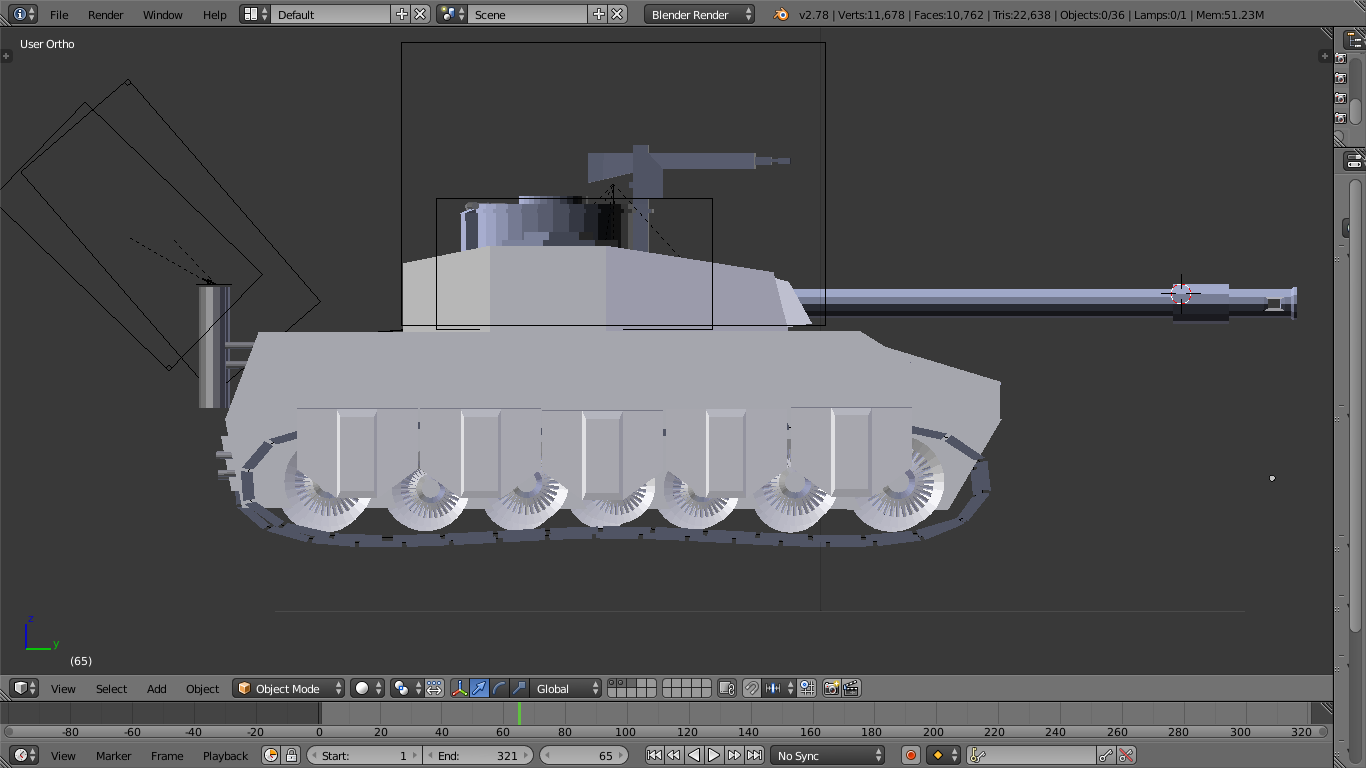
\includegraphics[width=10cm, height=8cm]{p1.png}
  \centering
  \caption{Perfil lateral do modelo do tanque após a modelação.}
  \label{fig:tanque1}
\end{figure}

\begin{figure}[!h]
  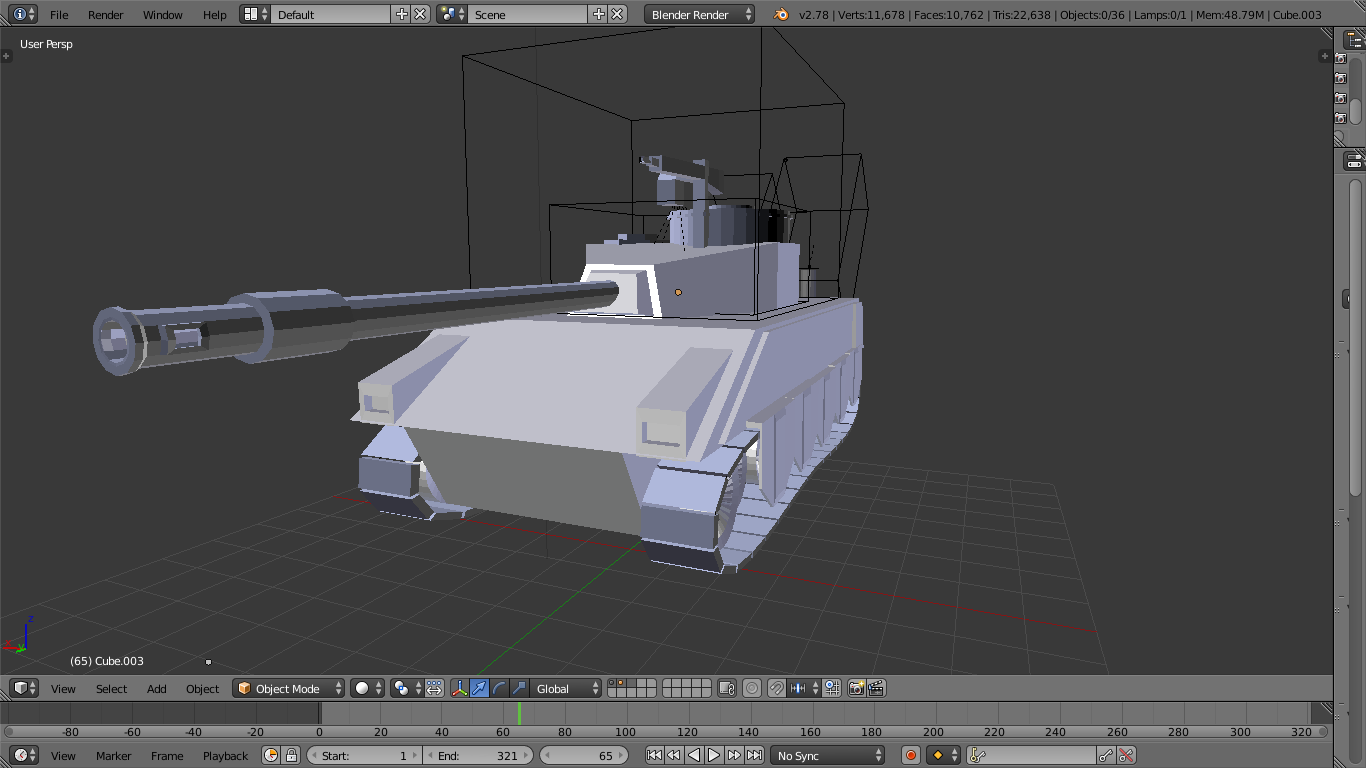
\includegraphics[width=10cm, height=8cm]{p2.png}
  \centering
  \caption{Perfil lateral do modelo do tanque após a modelação.}
  \label{fig:tanque2}
\end{figure}

\begin{figure}[!h]
  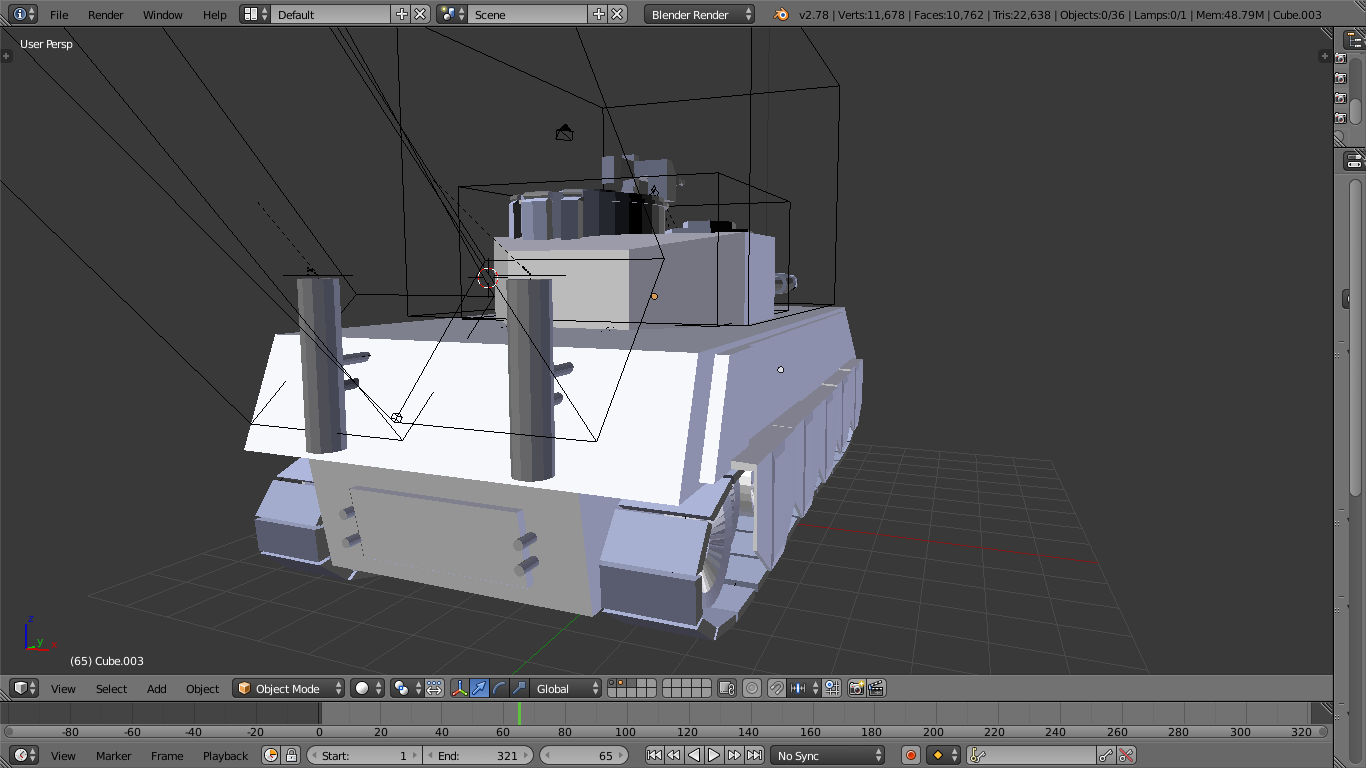
\includegraphics[width=10cm, height=8cm]{p3.png}
  \centering
  \caption{Perfil da retaguarda do modelo do tanque após a modelação.}
  \label{fig:tanque3}
\end{figure}

\begin{figure}[!h]
  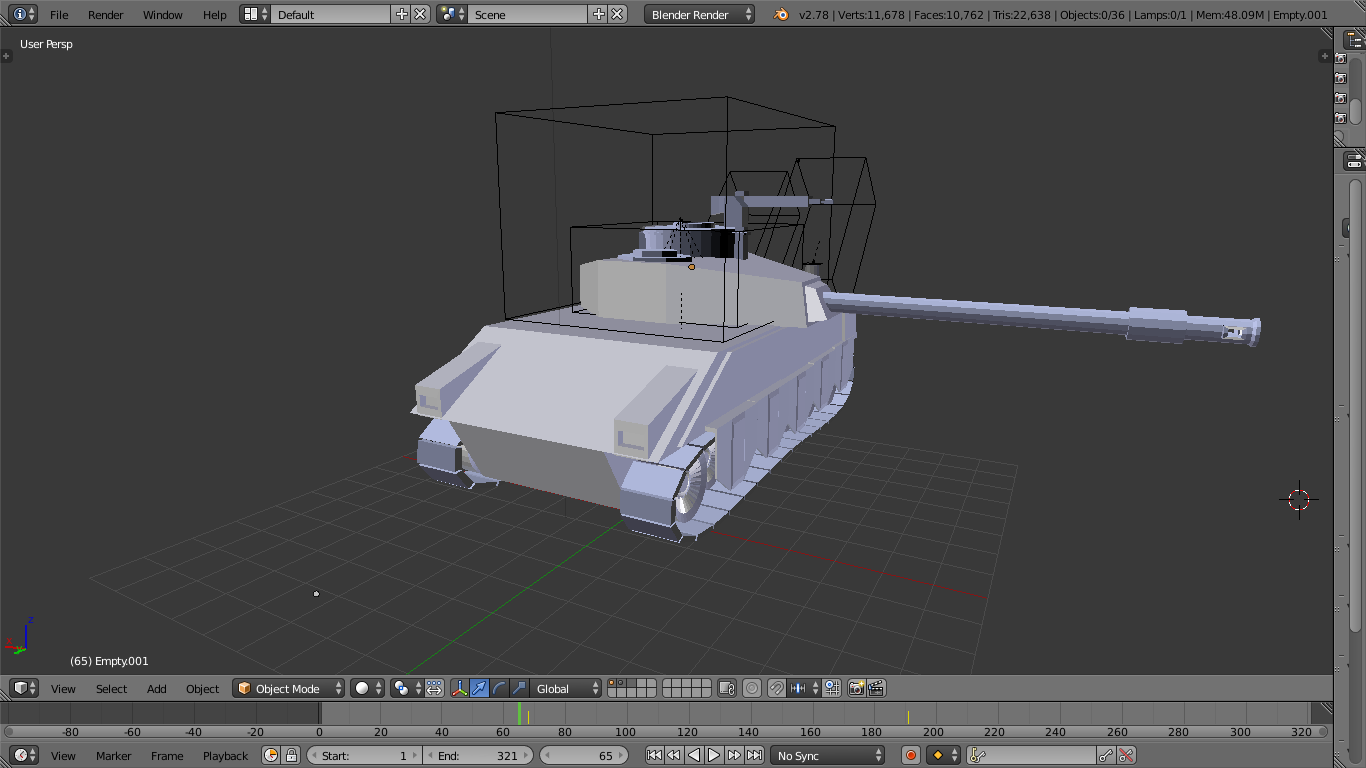
\includegraphics[width=10cm, height=8cm]{p4.png}
  \centering
  \caption{Perfil frontal com a lateral da torre do modelo do tanque após a modelação.}
  \label{fig:tanque4}
\end{figure}

\begin{figure}[!h]
  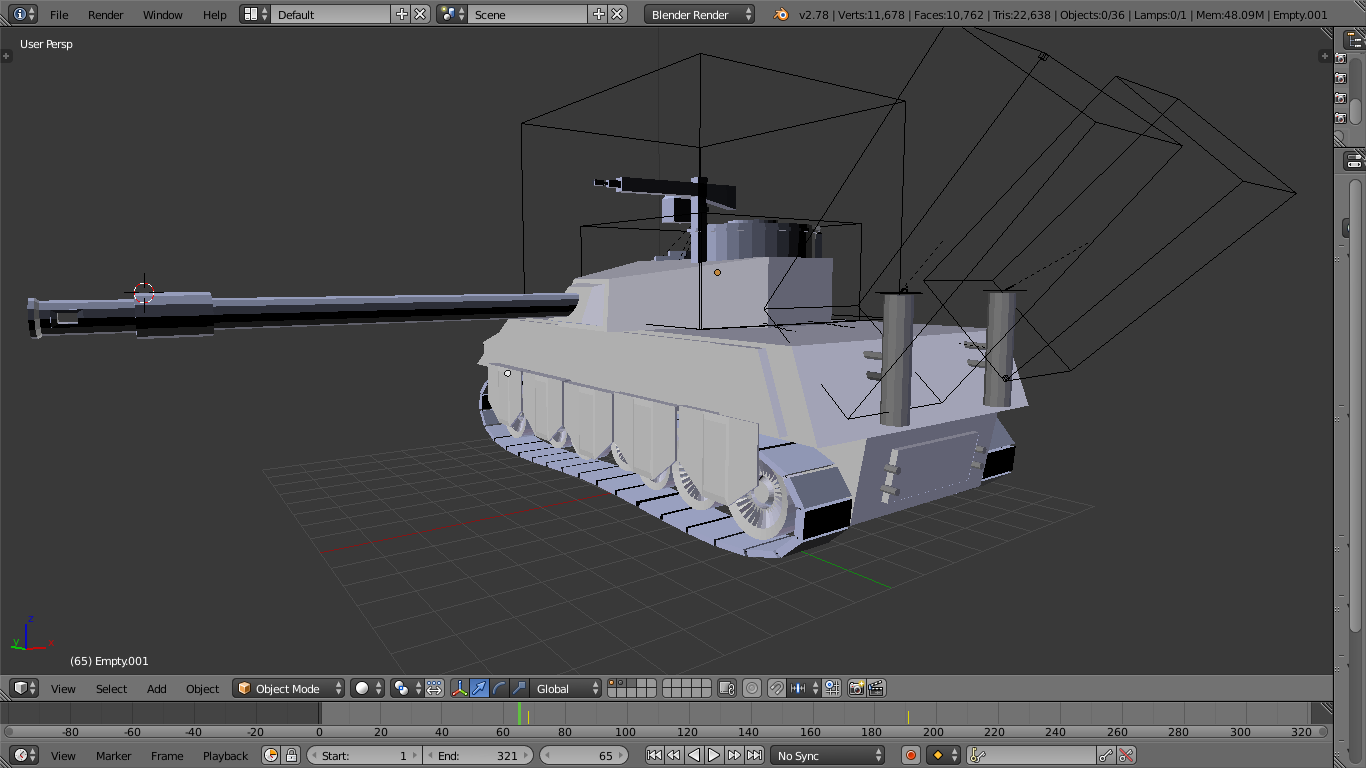
\includegraphics[width=10cm, height=8cm]{p5.png}
  \centering
  \caption{Perfil da retaguarda com a lateral da torre do modelo do tanque após a modelação.}
  \label{fig:tanque5}
\end{figure}

O aspeto visual dos modelos nesta fase de desenvolvimento não difere o suficiente para fazer com que seja necessário mostrar todas estas imagens de perfil para os três modelos, de maneira que apenas são mostradas para o tanque.
Tendo esta forma, procedeu-se a fazer a aplicação de texturas e à iluminação do modelo. \\ 

A aplicação de texturas foi feita de forma simples, usando cores básicas e adicionando apenas algum fator de granularidade nas formas, de maneira a parecer que os modelos tinham uma dimensão de textura que, na realidade, não tinham.
A iluminação foi aplicada usando composição, sendo que o seu ponto inicial, direção e características de força foram alteradas para que nenhuma parte do modelo estivesse escura, mas mantendo a parte frontal mais brilhante que o resto.
Foi então adicionado o fundo, inspirado numa floresta, criado seguindo as guias descritas em cima, referentes aos modelos, utilizado para todos os outros modelos. \\ 

Após esta fase, foi feita a produção dos efeitos de simulação do disparo do veículo e a sua animação (tanto do modelo como dos efeitos de disparo e fumo inseridos). A fase de animação mostrou ser complexa, o que levou a um estudo sobre a matéria. No conjunto, estas quatro fases (aplicação de texturas, iluminação, criação do fundo e animação) demoraram um total de uma semana, sendo que estas não foram tão detalhadas como a fase de modelação. \\ 

Tendo terminado a animação do modelo, foi feita a composição, mais uma vez, de todos os efeitos e iluminação de maneira a refletir o movimento do modelo. Foi então feita a pós-produção do vídeo, adicionando som e corrigindo cores e outros aspetos, de maneira a o tornar mais agradável de ser visualizado. As formas finais dos modelos aqui exibidas foram retiradas dos vídeos que foram produzidos, por isso têm compensação de cor e apresentam algum nível de granularidade, devido à compressão feita para manter os tamanhos dos ficheiros relativamente pequeno.\\ 

A forma final do modelo do tanque, depois de todo o desenvolvimento pode ver-se na figura \ref{fig:fff1}.
\begin{figure}[!h]
  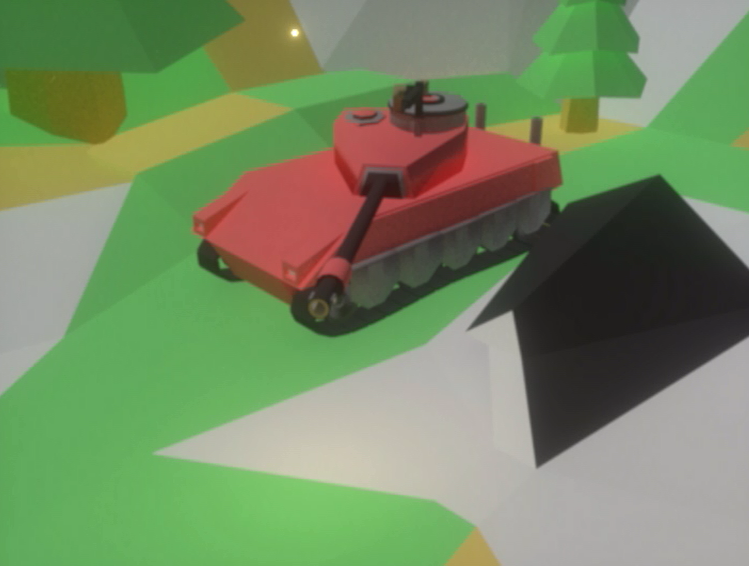
\includegraphics[width=10cm, height=8cm]{model4.png}
  \centering
  \caption{Forma final do modelo do tanque após o seu desenvolvimento.}
  \label{fig:fff1}
\end{figure}

Depois do tanque, foi feito o desenvolvimento do vídeo para uma peça de artilharia. Este desenvolvimento difere do tanque no sentido em que tentei simplificar ainda mais as formas utilizadas, focando mais na animação e composição da aparência depois de modelado. 
Esta abordagem resultou num modelo com uma aparência mais simples, mas que criava a sensação de ser mais complexo que o anterior, especialmente levando em conta os efeitos adicionados depois da modelação.

\clearpage
A forma final do vídeo da artilharia após o seu desenvolvimento pode ver-se na figura \ref{fig:artilharia2}.


\begin{figure}[!h]
 \centerline{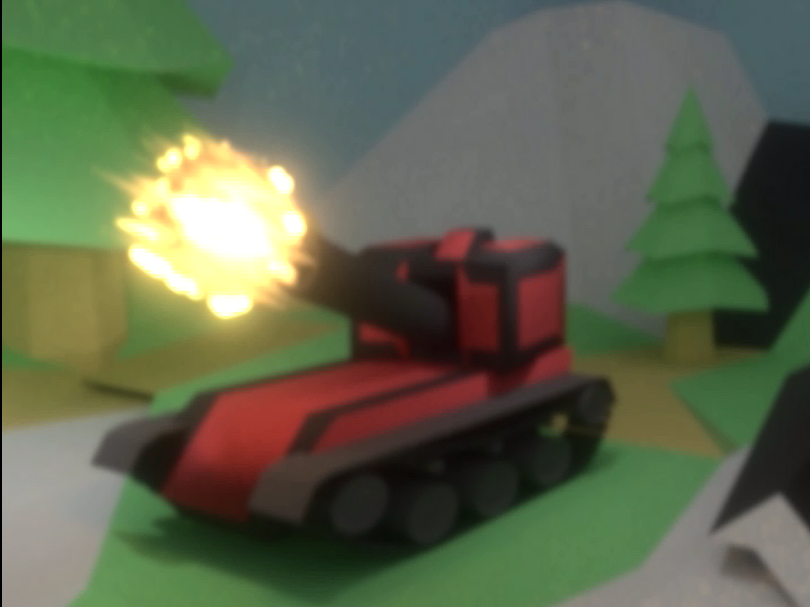
\includegraphics[width=10cm, height=8cm]{model2.png}}
  \centering
  \caption{Forma final do modelo da artilharia após o desenvolvimento.}
  \label{fig:artilharia2}
\end{figure}


Após o desenvolvimento da artilharia, foi iniciado o desenvolvimento do jipe, sendo este o modelo mais complexo e onde o detalhe da composição de efeitos é maior. Por causa disto, é o modelo mais agradável de ver mas também o mais complexo e de maior dimensão em termos de dados, demorando um total de três horas para completar a criação do vídeo (\textit{render} com animação e composição). \\

A forma final do jipe após o desenvolvimento pode ver-se na figura \ref{fig:jipe2}.

Com o desenvolvimento do jipe, acaba a fase em que é usada a ferramenta \emph{Blender}. Após a criação dos modelos e da sua animação é usado o motor de jogo \emph{Unity}, de maneira a os implantar no jogo. 

\begin{figure}[!h]
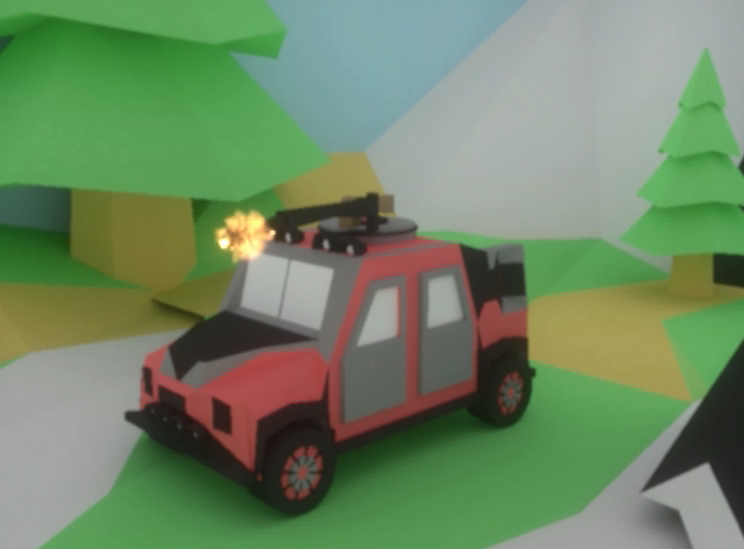
\includegraphics[width=10cm, height=8cm]{model6.png}
  \centering
  \caption{Forma final do modelo do jipe após o desenvolvimento.}
  \label{fig:jipe2}
\end{figure}

Com isto, acaba o desenvolvimento utilizando o \emph{Blender}.
\clearpage
\section{Unity}
\label{chap3:sec:unity}
Nesta secção, vai ser explicado no que consiste a ferramenta \emph{Unity}, as suas funcionalidades e capacidades assim como porque é que é uma opção de qualidade para o desenvolvimento de jogos de vídeo, quer em plataforma móvel quer em plataformas fixas.
\subsection{Funcionalidades e capacidades}
\label{chap3:subsec:funcionalidadesU}
O \emph{Unity} [15] é um motor de jogo \textit{cross-platform} utilizado no desenvolvimento de jogos de vídeo, simulações ou \textit{software} que lide com gráficos complexos. As suas funcionalidades vão desde a visualização de interfaces com gráficos embutidos até modelos de colisão e de física complexos para serem utilizados e gerados a tempo real, tais como simulações de fumo ou fluídos e a inserção de sombras dinâmicas e modelos de iluminação 3D. \\ 

Sendo \textit{cross-platform}, é possível desenvolver aplicações que usam o motor de jogo para um grande número de plataformas, como \emph{Windows}, \emph{Linux}, \emph{Android}, \emph{iOS} e várias consolas.


\subsection{Experiência}
\label{chap3:subsec:experienciaU}
Como aconteceu com a ferramenta Blender, a experiência com a ferramenta Unity era inexistente, onde a necessidade de aprendizagem constitui um fator importante para se conseguir produzir um conteúdo com qualidade satisfatória para ser apresentado na aplicação. Neste caso, a aprendizagem foi um pouco mais rápida que no \emph{Blender}, tendo, mesmo assim, certas dificuldades como a familiarização com a interface, a criação e importação de \textit{assets} e a própria linguagem de programação utilizada para a criação dos \textit{scripts}. Para o processo de aprendizagem, foi utilizado o manual de referência do \emph{Unity} [18]. \\ 

A linguagem de programação escolhida foi \emph{C\#}, sendo que também tinha como opção utilizar \emph{JavaScript}. No entanto, e contado com experiência anterior na utilização de \emph{Java}, foi uma transição relativamente direta para \emph{C\#}, sendo que também se trata de uma linguagem orientada a objetos.

A ligação dos vários componentes gráficos com a mecânica do jogo pretendida é feita através de \textit{scripts}, que são ligados a objetos complexos, chamados \emph{GameObject}'s. Esta ligação permite a utilização de funções e propriedades próprias a um determinado \emph{GameObject} (por exemplo, um \emph{GameObject} do tipo botão tem funcionalidades e propriedades diferentes de um \emph{GameObject} de imagem). \\ 

A utilização da ferramenta foi bastante direta e intuitiva, havendo apenas alguns detalhes que causaram alguns problemas, como o modo de emulação da rede ou as propriedades de visualização da aplicação.

Em termos da ligação entre os dois dispositivos foi feita com base na informação presente na guia de ligações do \emph{Unity} [15].

\section{Conclusão}
\label{chap3:sec:conc}
Com o trabalho desenvolvido neste capítulo, foram aprendidas diversas metodologias e ganhadas várias ideias de como é feito o desenvolvimento de videojogos utilizando as ferramentas referidas, podendo estas experiências traduzir-se em conhecimento que é utilizado em base diária em estúdios de criação da indústria. \\ 
Agora, tendo como base as explicações que foram dadas neste capítulo acerca das funcionalidades e características das ferramentas utilizadas, é possível seguir para a explicação do processo de desenvolvimento da aplicação em si, entrando em mais detalhe na estrutura da aplicação.